\begin{pa} \label{PA:11.8}  In the following questions, we investigate the two new coordinate systems that are the subject of this section:  cylindrical and spherical coordinates.  Our goal is to consider some examples of how to convert from rectangular coordinates to each of these systems, and vice versa.  Triangles and trigonometry prove to be particularly important.
\begin{figure}[ht]
\begin{center}
\begin{minipage}{2.5in}
\begin{center}
%\resizebox{!}{2.4in}{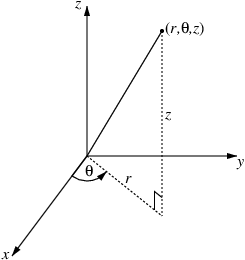
\includegraphics{11_8_Cylindrical_coords}}
  
\includegraphics{figures/fig_11_8_cylindrical.eps}
\end{center}
\caption{The cylindrical coordinates of a point.}
\label{F:11.8.Cylindrical_coords}
\end{minipage} \hspace{0.5in}
\begin{minipage}{2.5in}
\begin{center}
%\resizebox{!}{2.4in}{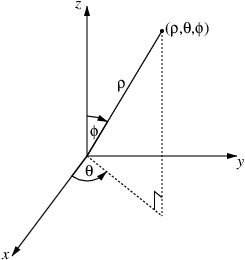
\includegraphics{11_8_Spherical_coords}}
  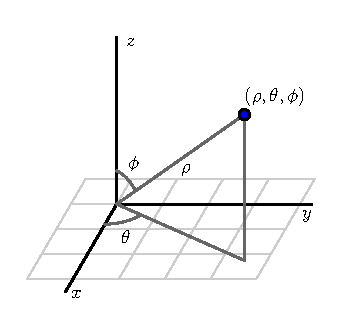
\includegraphics{figures/fig_11_8_spherical.eps}
\end{center}
\caption{The spherical coordinates of a point.}
\label{F:11.8.Spherical_coords}
\end{minipage}
\end{center}
\end{figure}

\noindent The cylindrical coordinates of a point in $\R^3$ are given by $(r,\theta,z)$ where $r$ and $\theta$ are the polar coordinates of the point $(x, y)$ and $z$ is the same $z$ coordinate as in Cartesian coordinates. An illustration is given in Figure \ref{F:11.8.Cylindrical_coords}.
    \begin{enumerate}
    \item[(a)] Find cylindrical coordinates for the point whose Cartesian coordinates are $(-1, \sqrt{3}, 3)$. Draw a labeled picture illustrating all of the coordinates.


	\item[(b)] Find the Cartesian coordinates of the point whose cylindrical coordinates are $\left(2, \frac{5\pi}{4}, 1\right)$. Draw a labeled picture illustrating all of the coordinates.	

	\end{enumerate}

\noindent The spherical coordinates of a point in $\R^3$ are $\rho$ (rho), $\theta$, and $\phi$ (phi), where $\rho$ is the distance from the point to the origin, $\theta$ has the same interpretation it does in polar coordinates, and $\phi$ is the angle between the positive $z$ axis and the vector from the origin to the point, as illustrated in Figure \ref{F:11.8.Spherical_coords}.  \\

\noindent For the following questions, consider the point $P$ whose Cartesian coordinates are $(-2,2,\sqrt{8})$.

\begin{enumerate}
     \item[(c)] What is the distance from $P$ to the origin?  Your result is the value of $\rho$ in the spherical coordinates of $P$.


     \item[(d)] Determine the point that is the projection of $P$ onto the $xy$-plane.  Then, use this projection to find the value of $\theta$ in the polar coordinates of the projection of $P$ that lies in the plane.  Your result is also the value of $\theta$ for the spherical coordinates of the point.



     \item[(e)] Based on the illustration in Figure \ref{F:11.8.Spherical_coords}, how is the angle $\phi$ determined by $\rho$ and the $z$ coordinate of $P$? Use a well-chosen right triangle to find the value of $\phi$, which is the final component in the spherical coordinates of $P$. Draw a carefully labeled picture that clearly illustrates the values of $\rho$, $\theta$, and $\phi$ in this example, along with the original rectangular coordinates of $P$.


     \item[(f)] Based on your responses to (c), (d), and (e), if we are given the Cartesian coordinates $(x,y,z)$ of a point $Q$, how are the values of $\rho$, $\theta$, and $\phi$ in the spherical coordinates of $Q$ determined by $x$, $y$, and $z$?

     

    \end{enumerate}

\end{pa} 

\begin{activitySolution} 

    \ba
    \item We know the $z$ coordinate is $3$. We also know that
\[r = \sqrt{(-1)^2 + (\sqrt{3})^2} = 2 \ \ \ \text{ and } \ \ \ \tan(\theta) = -\sqrt{3}.\]
Since the point $(-1,\sqrt{3})$ is in the second quadrant, we have $\theta = \frac{2\pi}{3}$. So a set of cylindrical coordinates for the point with Cartesian coordinates $(-1, \sqrt{3}, 3)$ is $\left(2, \frac{2\pi}{3}, 3\right)$.

	
	\item In this case we have $x = 2\cos\left(\frac{5\pi}{4}\right) = -\sqrt{2}$, $y =2\sin\left(\frac{5\pi}{4}\right) = -\sqrt{2}$, and $z=1$. 


    \item The distance from $P$ to the origin is
\[\rho = \sqrt{2^2+2^2+(\sqrt{8})^2} = 4.\]

     \item  The projection of the point onto the $xy$-plane is the point $(-2,2,0)$. So $\theta$ satisfies $\tan(\theta) = \frac{-2}{2}=-1$. Since this point is in the second quadrant we have $\theta = \frac{3\pi}{4}$.

     \item Here we have $\cos(\phi) = \frac{z}{\rho} = \frac{\sqrt{8}}{4} = \sqrt{2}{2}$. So $\phi = \frac{\pi}{4}$. Thus, spherical coordinates of the point $P$ are $\left(4, \frac{3\pi}{4}, \frac{\pi}{4}\right)$.  

     \item If we know the Cartesian coordinates $(x,y,z)$ of a point, then spherical coordinates $(\rho, \theta, \phi)$ of this point satisfy
\[\rho :=\sqrt{x^2+y^2+z^2}, \ \ \ \tan(\theta) = \frac{y}{x} \text{ provided } x\neq 0, \ \ \ \text{ and } \ \ \ \cos(\phi) = \frac{z}{\rho} \text{ provided } \rho \neq 0.\]

	\ea

\end{activitySolution}


\afterpa 